\section{Durchführung}
\label{sec:Durchführung}

Für die Messung wurde eine Grundplatte wie in \autoref{fig:Abb1} dargestellt benutzt. Genauere Daten der Probestäbe wurden in der \autoref{tab:werte2} angegeben.

\begin{figure}
    \centering
    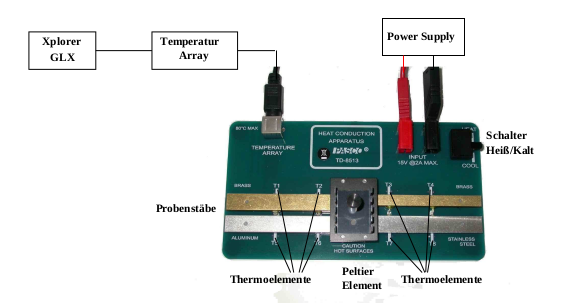
\includegraphics[scale=0.7]{content/Bilder/Aufbau.png}
    \caption{Hier zu sehen ist die für das Experiment verwendete Grundplatte, dessen Probestäbe im Verlauf des Versuchs aufgeheizt und abgekühlt wurden. Die einzelnen Bauteile sind hier beschrieben.}
    \label{fig:Abb1}
\end{figure}
\begin{table}
    \centering
    \caption{Hier ist eine Auflistung für die gegebenen Werte der Bauteile des Schwingkreises.}
    \label{tab:werte2}
    \begin{tabular}{c c c c}
        \toprule
        Material & Abmessungen [m] & \(rho\) [kg/$m^3$] & c [J/kg K] \\
        \midrule
            Messing (breit) & 0.09 x 0.012 x 0.004 & 8520 & 385 \\
            Messing (breit) & 0.09 x 0.007 x 0.004 & 8520 & 385 \\
            Aluminium (breit) & 0.09 x 0.012 x 0.004 & 2800 & 830 \\
            Edelstahl (breit) & 0.09 x 0.012 x 0.004 & 8000 & 400 \\
    \end{tabular}
  \end{table}

